\chapter{Machine Learning Background}
\label{cha:ML}

This chapter gives an introduction and explanation of several machine learning techniques and the theory behind them. The areas to be explored include: supervised learning, neural networks, convolutional neural networks and surrogate machine learning models. These methods require a data-set to perform meaningful analysis. This data-set will consist of many individual examples (or instances), e.g. an image, sound clip etc. whereas in the case of this research, an instance may be a single Parmec case.
\\

\noindent
For a more detailed explanation of the theory and workings of machine learning, see \cite{bishop2006pattern}.


\section{Supervised Learning} \label{supervised}

What defines supervised learning is the use of a data-set which has two parts: inputs (features) and outputs (labels, also known as ground truth or targets). The objective of supervised learning is to develop a model which can predict the labels using features which it has not seen before.
\\

\noindent
Supervised learning can be split into regression and classification. This section will focus on regression as it is more relevant to the work discussed in this paper. Regression concerns the prediction of a continuous variable through a mathematical combination of input variables. This contrasts with classification, which attempts to predict if a given sample belongs to a certain category or not.
\\

\noindent
Consider Figure~\ref{fig:boston} which shows 10 instances of the Boston house price data-set \cite{harrison1978hedonic} each representing houses in a metropolitan area. This table shows three features (highlighted in blue): RM (average number of rooms per dwelling), LSTAT (percentage of lower status residents) and PTRATIO (ratio of the pupils to teachers). In the final column, we see our target variable (green), which in this case represents median house price. 
\\

\noindent
In supervised learning practice, a model is trained to predict the target variable from values of the features: so in this case, the model would predict house prices based on the number of rooms, percentage of lower status residents and pupil-teacher ratio. 
\\

\begin{figure}[ht]
	\centering
	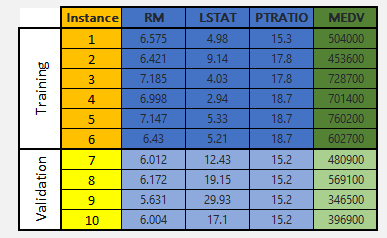
\includegraphics[scale=0.75]{Figures/boston.png}
	\caption{The Boston House Price Data-set (sample).}
	\label{fig:boston}
\end{figure}

\begin{equation} \label{feature_matrix}
	X \subseteq \mathbb{R}^{n \times f}
\end{equation}

\noindent
The features can be seen as a matrix X of real numbers with dimensions n by f (number of instances by number of features - (\ref{feature_matrix})). To generate a vector containing predicted target values ($\hat{y}$) from a feature matrix, the model performs the matrix operation as shown in (\ref{supervised_model}). The weights vector, w, as well as the bias value, b, are optimised through a process of training known as gradient descent. 
\\

\begin{equation} \label{supervised_model}
	X \times w + b = \hat{y}
\end{equation}

\noindent
To perform gradient descent, a difference metric is calculated between the predicted values, $\hat{y}$ and the true target values, y (e.g. the final column of Figure~\ref{fig:boston}). There are many loss functions that can be  used to calculate this metric, with a common one being the mean-squared-error (MSE) equation as shown in (\ref{mse}).
\\

\begin{equation} \label{mse}
	MSE = \frac{1}{n}\sum_{i=1}^n [(x_i \times w + b) - y_i]^2
\end{equation}

\noindent
In (\ref{mse}), we see the square difference calculated on an instance-by-instance basis (i) between the prediction (left) and true label (right). The mean value is then used to update the weights by taking its derivative of the MSE with respect to each weight. Theoretically, there is a minimum value of MSE for each weight (j), though this value cannot be calculated explicitly. Instead, the loss is minimised through a process of iteratively adjusting the weights by the derivative of the MSE (Figure~\ref{fig:GRA}). This process is repeated for the entire data-set multiple times, with each iteration being called an epoch. The training process will be continued for a user defined number of epochs, until a specified loss is reached, or until model convergence has been reached i.e there is no further improvement in model performance.
\\

\noindent
Various loss functions are available, with common examples being the mean squared error (MSE) already mentioned, as well as mean absolute error (MAE) and the Huber loss \cite{huber1964robust}. At the end of training, another loss value can be calculated using the test set to evaluate the overall general performance of a given model and compare different approaches.   
\\

\noindent
The regression method described here is linear regression. Alternative ML approaches to regression include Support Vector Regression (SVR) \cite{awad2015support} and Decision Tree Regression \cite{loh2014classification}.


\begin{figure}[ht]
	\centering
	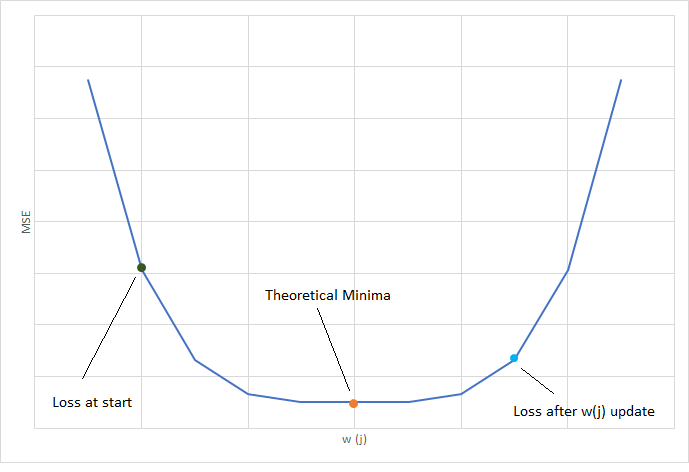
\includegraphics[scale=0.4]{Figures/gradient_descent.png}
	\caption{Gradient Descent}
	\label{fig:GRA}
\end{figure}

\section{Neural Networks} \label{NN}

Neural networks can be seen as a multi-layer stacking of the type of operation described in section~\ref{supervised}. The point at which each of these operations occurs is usually referred to as a neuron or node. Neurons are placed in parallel or sequence (Figure~\ref{fig:neural_network}) to form the model architecture.  Various arrangements of these nodes may be employed, with varying depth and width of the network. 
\\

\noindent
Differing neural network architectures with varying hyper-parameters \cite{gurney1997introduction} can be employed in the design of a machine learning surrogate model. The architecture of a neural network consists of nodes at which a mathematical operation is performed. The nodal output is passed through an activation function which transforms it in a non-linear manner. Commonly employed activation functions include the rectified linear unit (ReLu) \cite{hara2015analysis} and the Softplus function \cite{zheng2015improving}. 
\\

\noindent
The design of a neural network usually features multiple cascading layers, with the output of the previous layer feeding through as input to the subsequent layer. The network is trained through application of the back-propagation algorithm \cite{hecht1992theory} which uses the loss function to adjust the weights throughout the network. The back-propagation algorithm utilises a learning rate, a user defined value that determines how quickly the model weights are adjusted. A learning rate value must be chosen so as not be too high or low: either extreme will prevent an optimal solution from being attained. The learning rate may be adjusted during training. 
\\

\noindent
At the start of neural network training - prior to the back-propagation process - the trainable parameters of the model are initialised with random values. Repeating the initialisation and training process several times, a different set of optimised weights will be produced each time, despite using the same training data. To account for this stochastic nature of the training process, machine learning experiments are normally repeated several times.
\\

\noindent
A common problem encountered during the training of neural networks is that of overfitting \cite{hawkins2004problem}. This phenomenon is encountered when a model fits so closely to a training dataset that it does not perform well on new data that it has not encountered during training i.e. the model does not generalise well. A significantly lower training loss relative to the test loss indicates overfitting, whereas a similar value for the two loss values indicates good general performance of the model. To avoid overfitting, several regularisation techniques are employed. These include adding a term to loss function that penalises large weights and randomised dropout of model layers \cite{srivastava2014dropout}. 
\\

\noindent
Several configurations of neural networks are available. A common choice is the fully connected or dense neural network (DNN): i.e. the output of every node in a layer feeds into every node in the subsequent layer, leading to a 'dense' architecture. This configuration was employed in the aforementioned research papers. An alternative configuration is the convolutional neural network (CNN) discussed in the following chapter. 

\begin{figure*}[p]
	\centering
	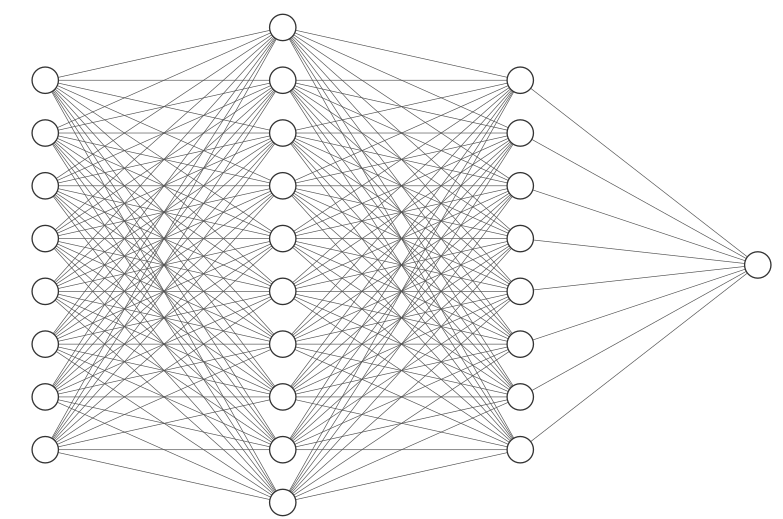
\includegraphics[scale=0.6]{Figures/nn.png}
	\caption{Neural Network: An example of a feed-forward network.} {From left to right: input layer accepting 8 features; first 'hidden' layer with 10 nodes, each fully connected to every node in the previous layer; second 'hidden' layer this time with only 8 nodes, again is fully connected to accept the output of each node from the previous layer; a single output node which is fully connected to each node from the previous layer.}
	\label{fig:neural_network}
\end{figure*}

\begin{figure*}[p]
	\centering
	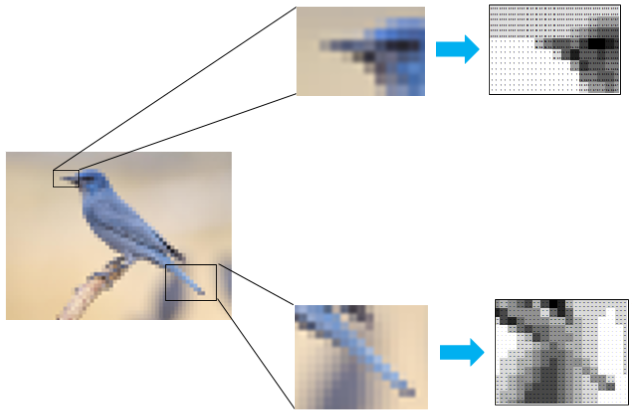
\includegraphics[scale=0.75]{Figures/cnn_feature.png}
	\caption{Convolutional Neural Network: Feature Extraction.}
	\label{fig:cnn_feature}
\end{figure*}

\section{Convolutional Neural Networks (CNN)} \label{convolution}

Convolutional neural networks (CNNs) attempt to capture local signals in data by use of a sliding window which passes over the input space. The application of CNNs may be effective in our work as there are similarities between the data format for AGR graphite core analysis and image recognition, with the presence and identification of local arrangements important in both areas. CNNs have been utilised in several areas of image analysis, including cell detection in medicine \cite{xie2015beyond} and depth estimation in photographs \cite{li2015depth}. Within the engineering field, they have been employed to predict remaining useful life of components \cite{babu2016deep}.
\\

\begin{figure*}[p]
	\centering
	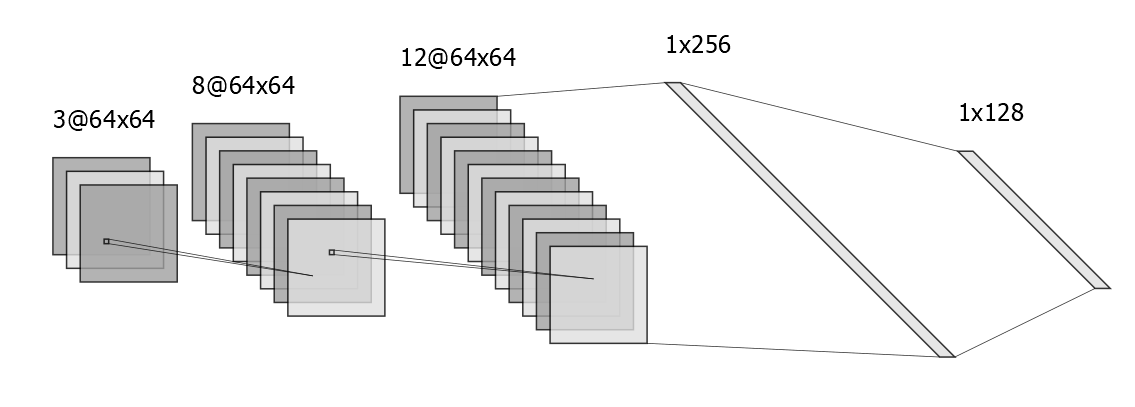
\includegraphics[scale=0.45]{Figures/cnn_arch.png}
	\caption{Convolutional Neural Network: Architecture.}
	\label{fig:cnn}
\end{figure*}

\section{Surrogate Machine Learning Models} \label{Surrogate}

For any given natural phenomena, it is possible to develop a physical model that mathematically describes it and can approximate its behaviour. Such phenomena range from a simple decaying wave (Figure~\ref{fig:surrogate}) to highly complex models such as that of turbulent fluid movement. Such models are unlikely to ever be a perfect representation of the natural phenomena, as there may be too many variables and factors to ever account for them all, hence there will always be some disparity. However, the model is likely to be accurate enough as to provide data that is of practical use.
\\

\noindent
From  data generated by such mathematical models, it is possible to train machine learning models to produce equivalent outputs from the same inputs. This will effectively be an additional layer of approximation on top of an already approximate model.
\\

\noindent
What is the motivation for doing this? Given a mathematical model of a phenomena, why develop and use a surrogate model using machine learning which provides inferior results? It is difficult to see why given the simple example of Figure~\ref{fig:surrogate}. However, in a real world case, such as nuclear reactor core safety, such a model may be highly complex, involving thousands of parameters and requiring significant computational expense. A machine learning model on the other hand, once trained, is computationally cheap to use, being just a series of matrix operations. The production of such a machine learning surrogate can also be seen as an exploration of the data space i.e. it is likely through the process of model training and refinement that insights into relationships between variables will be discovered. It may also be possible to develop machine learning tools so as to work in symbiosis with traditional mathematical models, with one informing the direction and focus of the other.



\begin{figure*}[p]
	\centering
	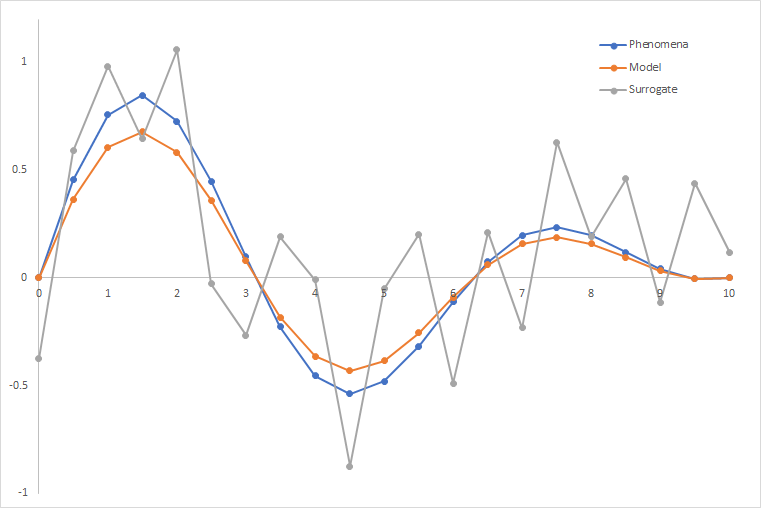
\includegraphics[scale=0.65]{Figures/surrogate_model.png}
	\caption{Modelling of Natural Phenomena} {A decaying wave (blue). A mathematical model may be developed which approximates its behaviour (orange). It may be possible to build a surrogate model (grey) which is an approximation built upon an approximation.}
	\label{fig:surrogate}
\end{figure*}

\section{Relevant Literature}

An overview of machine learning techniques and their application to nuclear engineering is given in a recent paper \cite{gomez2020status}. This review details a range of machine learning approaches, including decision trees, nearest-neighbour, support vector machines, naive bayes, as well as Convolutional and recurrent neural networks. It then goes on to outline how these techniques have been applied in nuclear engineering fields such as plant health, radiation protection and optimisation. Although this paper does not reference the AGR or graphite, it does provide a useful introduction to the field. 
\\

\noindent
The same authors produced an earlier paper in which they use a neural network to predict the response of a light water reactor to various operational and accident conditions \cite{fernandez2017nuclear}. The motivations for this work include an ability to make rapid safety decisions (i.e. greater computational efficiency) as well as providing insight into safety issues. This research highlights various neural network architectures as shown in Figure~\ref{fig:architectures}.  
\\

\begin{figure*}[p]
	\centering
	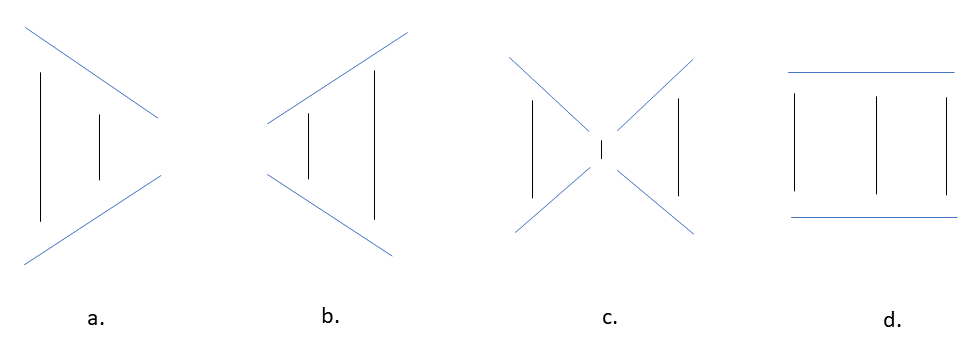
\includegraphics[scale=0.5]{Figures/architecture.png}
	\caption{Four Possible Neural Network Architectures} {Input on the left, output on the right. \textbf{(a)}: a narrowing structure where layers decrease in size towards the output layer and the output vector is smaller than the input vector; \textbf{(b)}: the inverse of a. with the layers increasing in size towards the output layer; \textbf{(c)}: An architecture combining both of the previous approaches, with the structure compressing the input and then expanding it before the output layer; \textbf{(d)}: A parallel structure where the layers remain of roughly similar size across the network. This Figure is a reproduction of Fig. 4 from \cite{fernandez2017nuclear}.}
	\label{fig:architectures}
\end{figure*}

\noindent
Academic works which apply machine learning to the production of engineering surrogates can be found as far back as 2003, where \cite{javadi2003neural} developed a symbiotic approach combine finite element models and neural network architecture. A more recent treatment of this topic can be found in \cite{kim2019machine} where the authors employ several approaches. These include an adaptive sampling method, where instances are generated and included in the training set based on their importance: i.e. selecting samples within the problem space that maximise useful information and excluding those which contain redundancy. Another relevant work is \cite{zeng2018machine} which uses a machine learning model to predict subsequent molten reactor core behaviour based on a time history. To train the ML model used in this work, the researchers generate data using a traditional engineering model (equivalent to that described in section \ref{Engineering}) to build a surrogate model (as described in section \ref{Surrogate}).  
\\

\noindent
A particularly relevant existing work to this research paper is \cite{dihoru2018neural} which concerns both AGR graphite and machine learning. These researchers use data from a physical model of an AGR reactor which simulates an earthquake to train a feed-forward neural network (see Figure~\ref{fig:neural_network}) with 3 layers. The data generated by five configurations of the physical model (one intact, four with random distributions of cracks) are used to generate values for displacement in the top layer of the core. A neural network is then trained on this data, with displacements in the central channel being used to predict displacements in a select number of surrounding channels. The researchers achieve reasonably good agreement between model prediction and the ground truth data from their physical model, although there is some breakdown at the extremes. The scope of this model is somewhat limited, however, in that the model can only predict displacements from displacements at other locations. Superior model performance may also be achieved with a more complex neural network.  
